\documentclass[a4paper,10pt]{article}
\usepackage[utf8]{inputenc}
\usepackage{graphicx}
\usepackage{booktabs}
\usepackage{rotating}
\usepackage{subfigure}
\usepackage{indentfirst}
\usepackage{float}
\us	epackage{cite}
\usepackage{/home/max/Dropbox/FMDV_AMERICA/PAPER/xcite} % Cite stuff from the main text
\usepackage{amsmath}
\bibliographystyle{plos2009}%
%%% Supp Mat modifications
\renewcommand{\thetable}{S\arabic{table}}   
\renewcommand{\thefigure}{S\arabic{figure}}
\externalcitedocument[M-]{FMDV_AMERICA}
%%%
%opening
\title{Text S2 -- Assessing the impact of taxon sampling on phylogeographic and coalescent reconstructions} % aargh, lousy name
\author{
Luiz Max Fagundes de Carvalho,
Guy Baele,
Nuno Rodrigues Faria,\\
Andres M. Perez,
Marc Suchard,
Philippe Lemey and
Waldemir de Castro Silveira
\\}
\date{}

\begin{document}

\maketitle

\section{Background}

The data sets used in this study presented preferential sampling, with some countries being overrepresented.
Namely, $58$ of the $131$ ($44.2\%$) sequences collected for serotype A were from Argentina, and $90$ of the $167$ ($53.9\%$) sequences for serotype O came from Ecuadorian isolates.
This unbalanced design may introduce bias on our phylogeography analysis, since under a null 'single rate' model, the more sequences are collected from a location, the higher the estimates to and from this location will be. % TODO: citation or formula here
% To see this, let....

Sampling bias constitutes an important concern in phylogeographic modeling, and several studies have performed sensitivity analyses to determine how robust inference is to biased sampling \cite{M-Faria2012,M-Lemey2013,M-polar,M-fluPNAS}.
Proposed approaches include using equally sampled data sets, for which each location contributes the same number of sequences \cite{M-fluPNAS}.
This approach is specially useful when a reasonable number of sequences is available.
Another strategy is to devise prior distributions for the CTMC infinitesimal rate matrix ($\mathbf{Q}$) that explicitly counteract the effects of biased sampling \cite{M-Faria2012}.

%TODO: talk about bias in skyride 

In this study we provide a thorough assessment of the effects of sampling bias in the phylogeographic inference results. 
First we propose a formal Bayesian test to gain insight into the effect of sampling bias, using the differences in representation as a predictor to viral spread.
Secondly, a customized sampling scheme is used to down-sample the original data sets and reduced representation bias.

\section{``Representation-informed'' priors and Country base frequencies}
The first experiment to study the impact of sampling in our estimated was to use what we call a ``representation-informed'' prior.
This prior is built by assuming that the average rate of flow between two locations is proportional to the difference in representation, i.e., the number of sequences from each location.
We can mathematically express the above rationale as:
\begin{equation}
\label{seq:repprior}
 m_{ij}=C\frac{|n_i-n_j|}{\sum_i|n_i-n_j|}
\end{equation}
where $n_i$ and $n_j$ are the number of sequences from locations $i$ and $j$ and $C$ is an arbitrary constant, chosen such that $E[m_{ij}]=1$ (see the Methods section in main text).
For each serotype we calculated marginal likelihoods using path sampling (PS) and stepping stone (SS) for the ``representation-informed'' priors.
These marginal likelihood were compared to the marginal likelihoods obtained using uniform prior distributions on the infinitesimal rate matrix.

We found Bayes factors of $200$ and $20$ between these models and their uniform counterparts for serotypes A and O respectively.
These results show significant statistical support for the ``representation-informed'' priors.

Also, we assessed the impact of fixed base frequencies for the locations, as follows: we allowed .
The 'fixed frequencies' analyses yielded substantially lower marginal likelihoods (data not shown, see main text for discussion).
Also, estimated base frequencies significantly differed from their observed counterparts as shown in Figure~\ref{sfig:freqs}.

\section{Robustness of parameter estimation and demographic reconstruction}

To quantify the impact of including older sequences, which are not available for all locations, we assessed the robustness of our temporal reconstruction by using only sequences from 2000 to present.
For this analysis, we used the Gaussian Markov Random Field (GMRF) smoothing prior on coalescent times, also known as `skyride' model.
These results are presented in Figure~\ref{sfig:only2000sky}.

Also, we were interested in studying whether overrepresented locations could influence phylogenetic parameter estimation.
To investigate that, we performed parameter estimation with and without these locations.
Tables~\ref{stab:SB_A} and~\ref{stab:SB_O} show medians and $95 \%$ credible intervals for several parameters of interest with and without the overrepresented locations
for both serotypes.
%%%%%%%%%%%%%%%%%%%%%%%%%%%
\subsection{Parameter estimation with down-sampling}

For large data sets it is possible to perform equal down-sampling, i.e., simple random stratified sampling \cite{M-fluPNAS}.
However, this was not possible in the data sets analyzed in this study.
The above experiments were performed by excluding all sequences from overrepresented locations.

To assess the effect of biased sampling while still using the information from overrepresented locations, we used a down-sampling scheme.
We draw as many sequences from the most represented location as there are sequences from the second most represented location.
For serotype A, the second most represented country was Venezuela ($27$ sequences) and for serotype O Colombia was the second location with more sequences ($36$).
To compose the subsamples for serotype A we then randomly drew $27$ sequences from Argentina and combined them to the other sequences in the original data set.
This procedure was performed five times to obtain five subsamples.
Sub-sampling for serotype O proceeded analogously.

Results of these experiments are presented in Tables~\ref{stab:ED_A} and~\ref{stab:ED_O}.
For most parameters there was substantial overlap between posterior distributions obtained using different subsamples.
Also, inference regarding the spatial origin (root) was consistent across subsamples for both serotypes.

\subsection{Comparing rate matrices}

A point of interest is whether the estimates for $\mathbf{Q}$ were consistent across subsamples.
First we plotted the estimated rates across each subsample against each other for both serotypes.
The results are shown in Figure~\ref{sfig:compz}A and~B and we can notice estimates are in agreement across subsamples.

We also calculated the $L_1$ matrix distance norm for (each pair of) the estimates of $\mathbf{Q}$ obtained from each subsample.
Let $\mathbf{X}$ and $\mathbf{Y}$ be two $K \times K$ square matrices.
The $L_1$ matrix norm is defined as

\begin{equation}
\label{seq:L1}
 L_1 = \frac{1}{K^{2} (\sum_{i=1}^{K^2} |X_i-Y_i| ) }
\end{equation}

Since all entries in our matrices are non-negative, we they were log-transformed prior to computing distances.
Calculations were performed using the \verb|norm()| in the \textbf{PET} package of the R statistical computing environment.
The results of these analyses are presented in Figure~\ref{sfig:compz}C and~D.

\subsection{Quantifying spatial signal extraction}
 In a Bayesian context, it is sometimes desirable to quantify how much information we gain from updating our prior information using the available data.
 A common measure of this signal extraction is the Kullback-Leibler (KL) divergence between prior and posterior distributions \cite{M-KL}.
 In a phylogeographic setting, Lemey et al. (2009) \cite{M-roots} propose to calculate the KL divergence between the posterior distribution for the states at root and a uniform discrete prior.
 Let $K$ be the number of discrete states (e.g. locations) and $\boldsymbol\theta$ be the $K$-dimensional vector of state probabilities.
 Then the prior density is
 \begin{equation}
 \label{seq:prior}
  \pi(\boldsymbol\theta_i) = \frac{1}{K} \quad \forall i \in \{1,..,K\} 
 \end{equation}
Next, let the trait data be denoted by $D$.
The posterior distribution of $\boldsymbol\theta$ is $p(\boldsymbol\theta|D)$.
The Kullback-Leibler divergence is given by:
\begin{equation}
 \label{seq:KL}
 \int p(\boldsymbol\theta|D)log\frac{p(\boldsymbol\theta|D)}{\pi(\boldsymbol\theta)}
\end{equation}
The higher the divergence, the more the posterior distribution is far away from its prior expectation, hence more signal is extracted from data.
We calculated equation~\ref{seq:KL} for the root state distributions for all subsamples (presented in Tables~\ref{stab:ED_A} and~\ref{stab:ED_O}) and all predictors (see main text).

\subsection{Spatial Bayesian Stochastic Search Variable Selection across subsamples}

In a phylogeographic setting, even for moderate numbers of locations we are usually left with the task of estimating a potentially large number of parameters. 
BSSVS seeks to select a parsimonious set of rates that sufficiently explain data variation.
By transforming each entry of the infinitesimal rate matrix $\mathbf{Q}$ into a vertex of the graph $\mathcal{G}$, the algorithm then searches the whole graph space, assigning an indicator variable $\delta_{ij}$ to each vertex.
Assuming each $\delta_{ij}$ is Bernoulli distributed with parameter $p_{ij}$, we can select only those entries with high probability of being included by BSSVS.
Using the fact that $\sum\delta_{ij}$ converges to a truncated Poisson distribution if the success probability is sufficiently small, we can can analytically compute Bayes factors using Equation 6 in Lemey et al. (2009).

To gain further insight into the impact of down-sampling in our phylogeographic inference, we conducted a Bayesian Stochastic Search Variable Selection (BSSVS) to search for the most parsimonious set of routes needed to explain data variation in each subsample.
As stated in the main text and in Lemey et al. (2009) \cite{M-roots}, this strategy naturally allows for the analytical calculation of Bayes factors for each migration route (i.e. graph edge).
BFs were then calculated for each subsample and plotted accordingly.
In Figure~\ref{sfig:bssvsA} we present the results for serotype A.
Results for serotype O are presented in Figure~\ref{sfig:bssvsO}.
For both serotypes a high degree of agreement between inferred significant routes between subsamples.
However, the distribution of states at root varies across subsamples.

For both serotypes the migration networks present two components; one connecting Venezuela, Colombia and Ecuador and another connecting southern cone countries, namely Brazil, Argentina and Uruguay.
Particularly, for serotype A we observe a supported migration routes between Venezuela and Brazil, which is absent from serotype O results.
Also, root probability distributions seem to be more consistent for serotype A than for serotype O.
\section{Discussion}
%\newpage
% A possibility, unexplored in this paper, is to sample each location with probability proportional to its disease prevalence
% In theory, a Bayesian approach should offer a certain degree of protection against model misspecification and sampling bias by bla  bla...
% robustness of skyride crap
\newpage
\section*{Figure Legends}
\textbf{Figure~\ref{sfig:freqs}. Estimated and observed trait (country) frequencies for both serotypes.}
We estimated base frequencies using a discrete uniform prior and compared the obtained median values to the observed frequencies for each country in each data set (serotype). 

\textbf{Figure~\ref{sfig:trade}. Exportation, importation and production time series for pigs, cattle and sheep in South America.}
Panel A shows exportations in log~(~\# ~of heads) of live animals for pigs, sheep and cattle.
Panels B and C show importation and overall production (population increase), respectively.

\textbf{Figure~\ref{sfig:tradeinfo}. Kernel density estimation for the trade-informed priors (predictors) used in this study.}
Information on cattle, sheep and pigs trade was retrieved from FAO and used to create trade-informed prior distributions for the CTMC infinitesimal rate matrix.
Each prior was evaluated for prior predictive probability (marginal likelihood) using the PS and SS algorithms. 

\textbf{Figure~\ref{sfig:AvsO}. Scatterplot of estimated rate matrices for serotypes A and O.}
We plotted all overlapping rates (Serotype O without Paraguay) estimated using a symmetric CTMC model for both serotypes, to investigate whether the two serotypes have different spatial patterns.

\textbf{Figure~\ref{sfig:compz}. Comparison of of estimated rate matrices across subsamples}
In panels A and B we show entry-wise scatterplots of the five subsamples for serotypes A and O respectively.
Colors depict country of origin.
Panel C and D shows heat maps of the $5\times5$ matrices of $L_1$ norms comparing each subsample, for serotypes A and O, respectively.

\textbf{Figure~\ref{sfig:bssvsA}. Bayesian Stochastic Search Variable Selection for five down-sampled subsamples of serotype A sequences.}
We performed the BSSVS analysis on five down-sampled data sets (reduced Argentina representation) and plotted the resulting Bayes factors.
Arrow thickness is proportional to Bayes factor magnitude and colors depict the probability of being root for each country.

\textbf{Figure~\ref{sfig:bssvsO}. Bayesian Stochastic Search Variable Selection for five down-sampled subsamples of serotype O sequences.}
We performed the BSSVS analysis on five down-sampled (equal numbers of Ecuadorian and Colombian sequences) data sets and  plotted the resulting Bayes factors.
Arrow thickness is proportional to Bayes factor magnitude and colors depict the probability of being root for each country.

\textbf{Figure~\ref{sfig:only2000sky}. Skyride coalescent reconstructions using sequences from 2000 to present only for both serotypes.}
As in the main text, disease cases and vaccination in doses per head are overlaid to the demographic reconstructions.

\newpage
\begin{center}
\begin{figure}[H]
\begin{center}
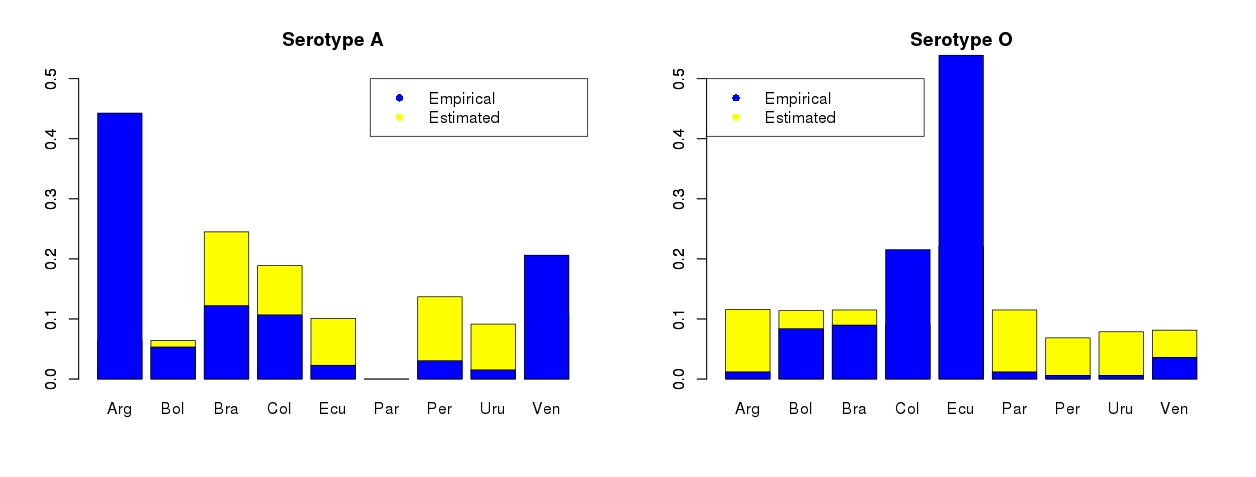
\includegraphics[scale=.35]{FIGURES/FMDV_frequencies_fixed.jpeg}
\end{center}
\caption{}
\label{sfig:freqs}
\end{figure}
\end{center}
\newpage
%%%%%%%%%%%%%%%%%%%
%%%%%%%%%%%%%%%%%%%
\begin{center}
\begin{figure}[H]
\begin{center}
\subfigure[A]{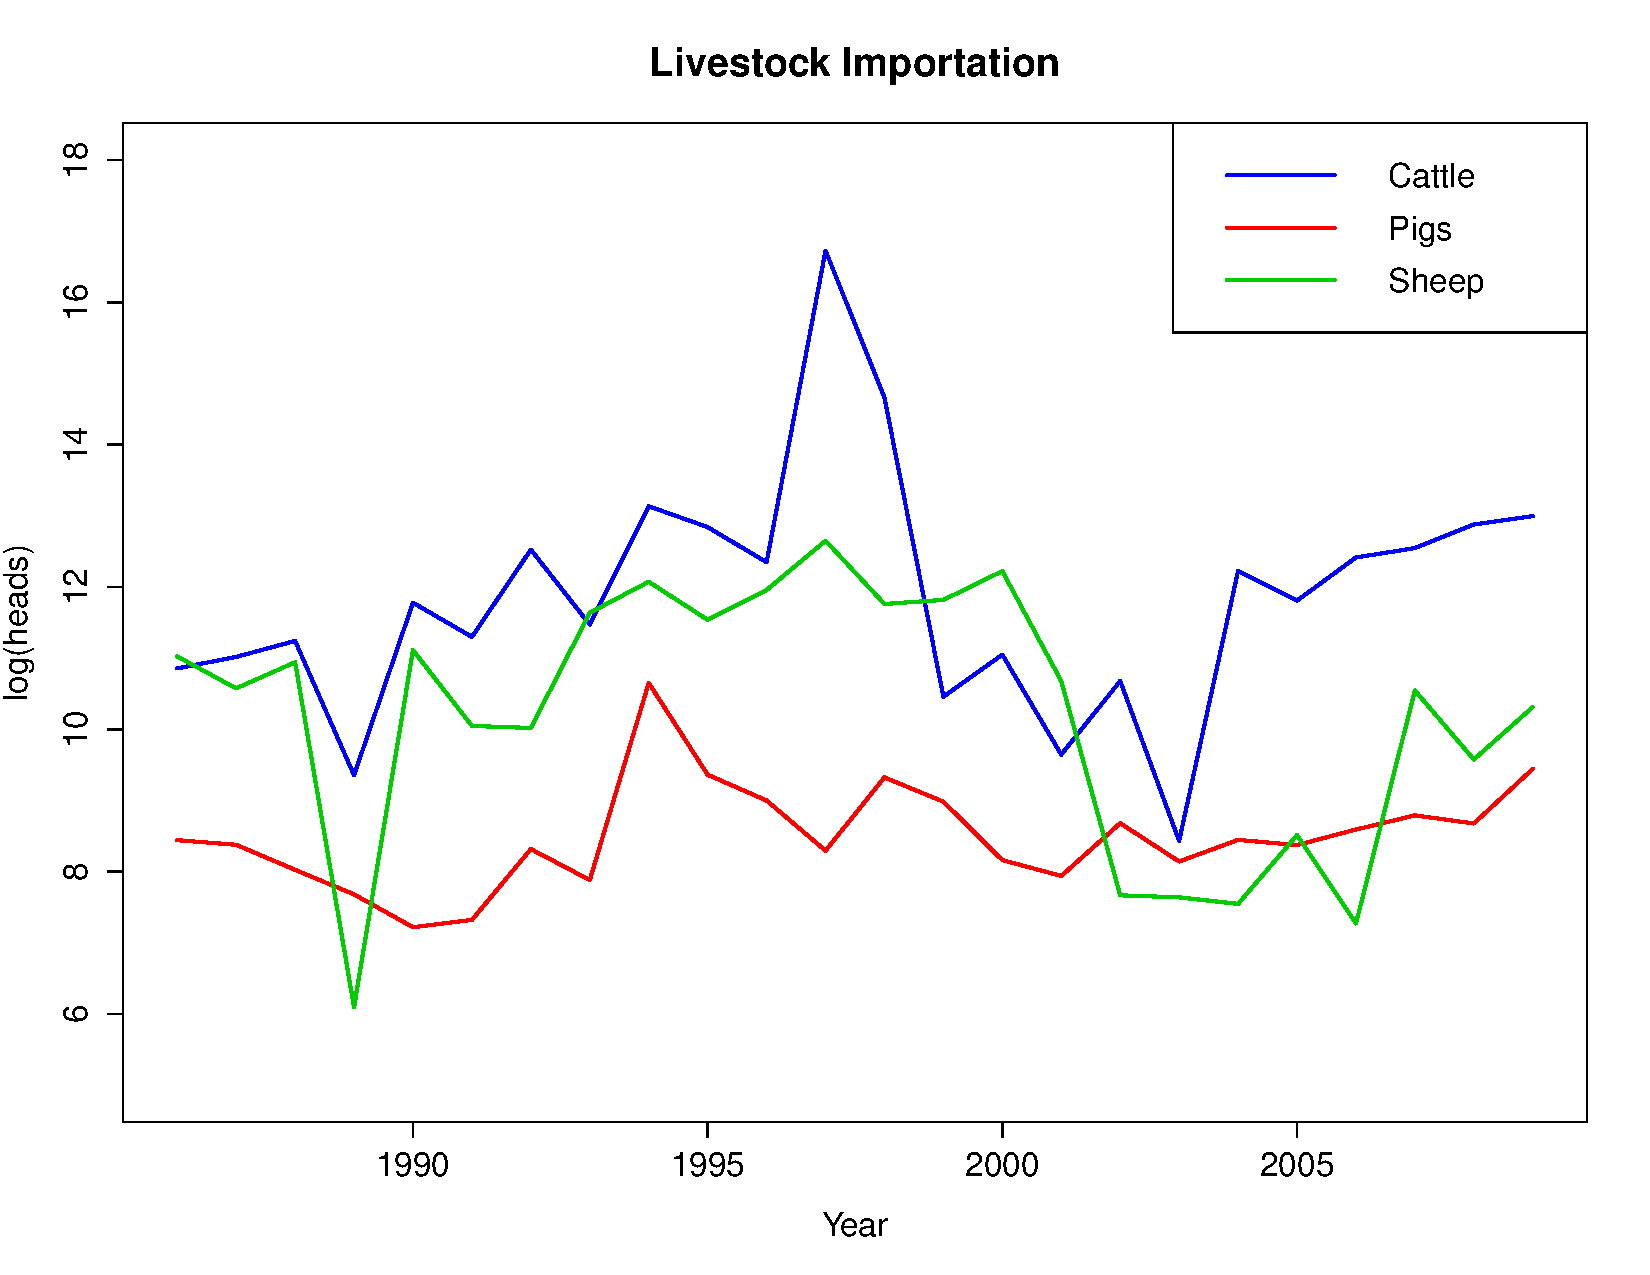
\includegraphics[scale=.250]{FIGURES/importation.pdf}}\\
\subfigure[B]{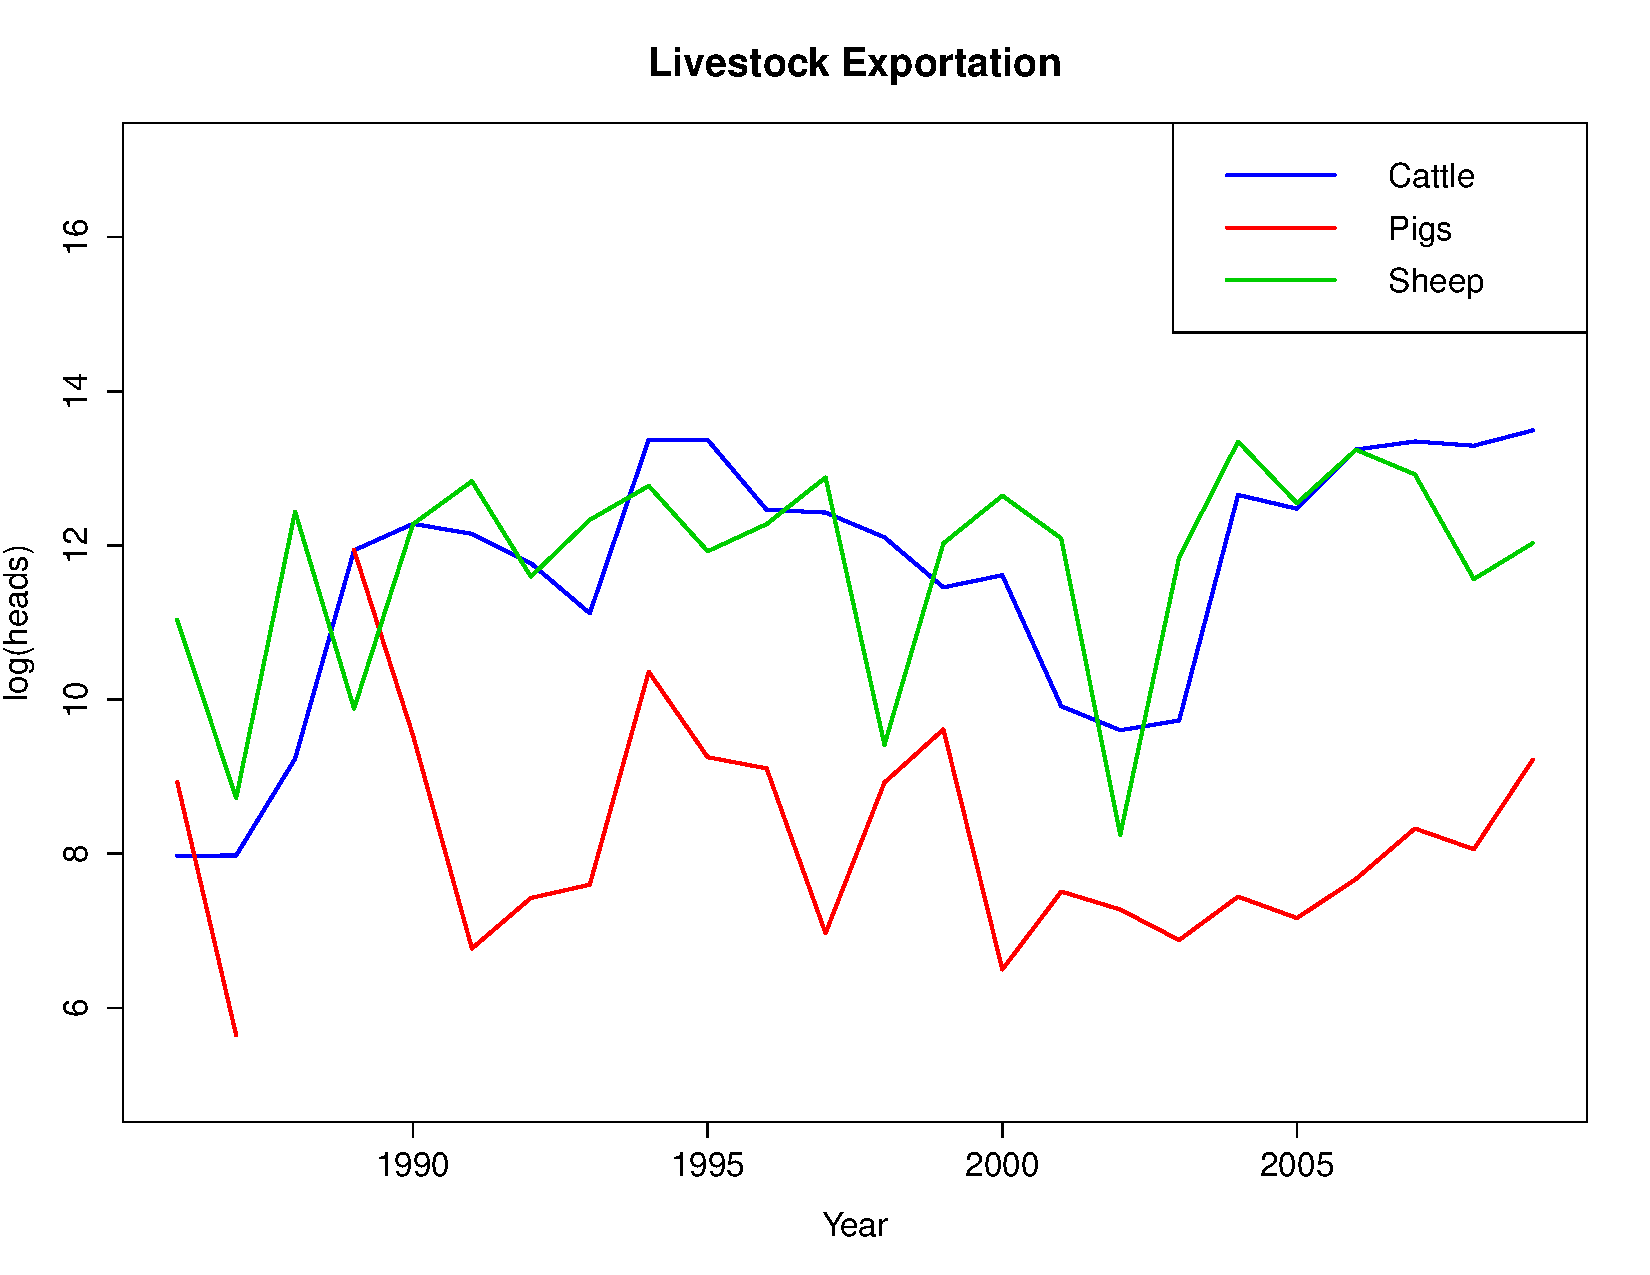
\includegraphics[scale=.250]{FIGURES/exportation.pdf}}\\
\subfigure[C]{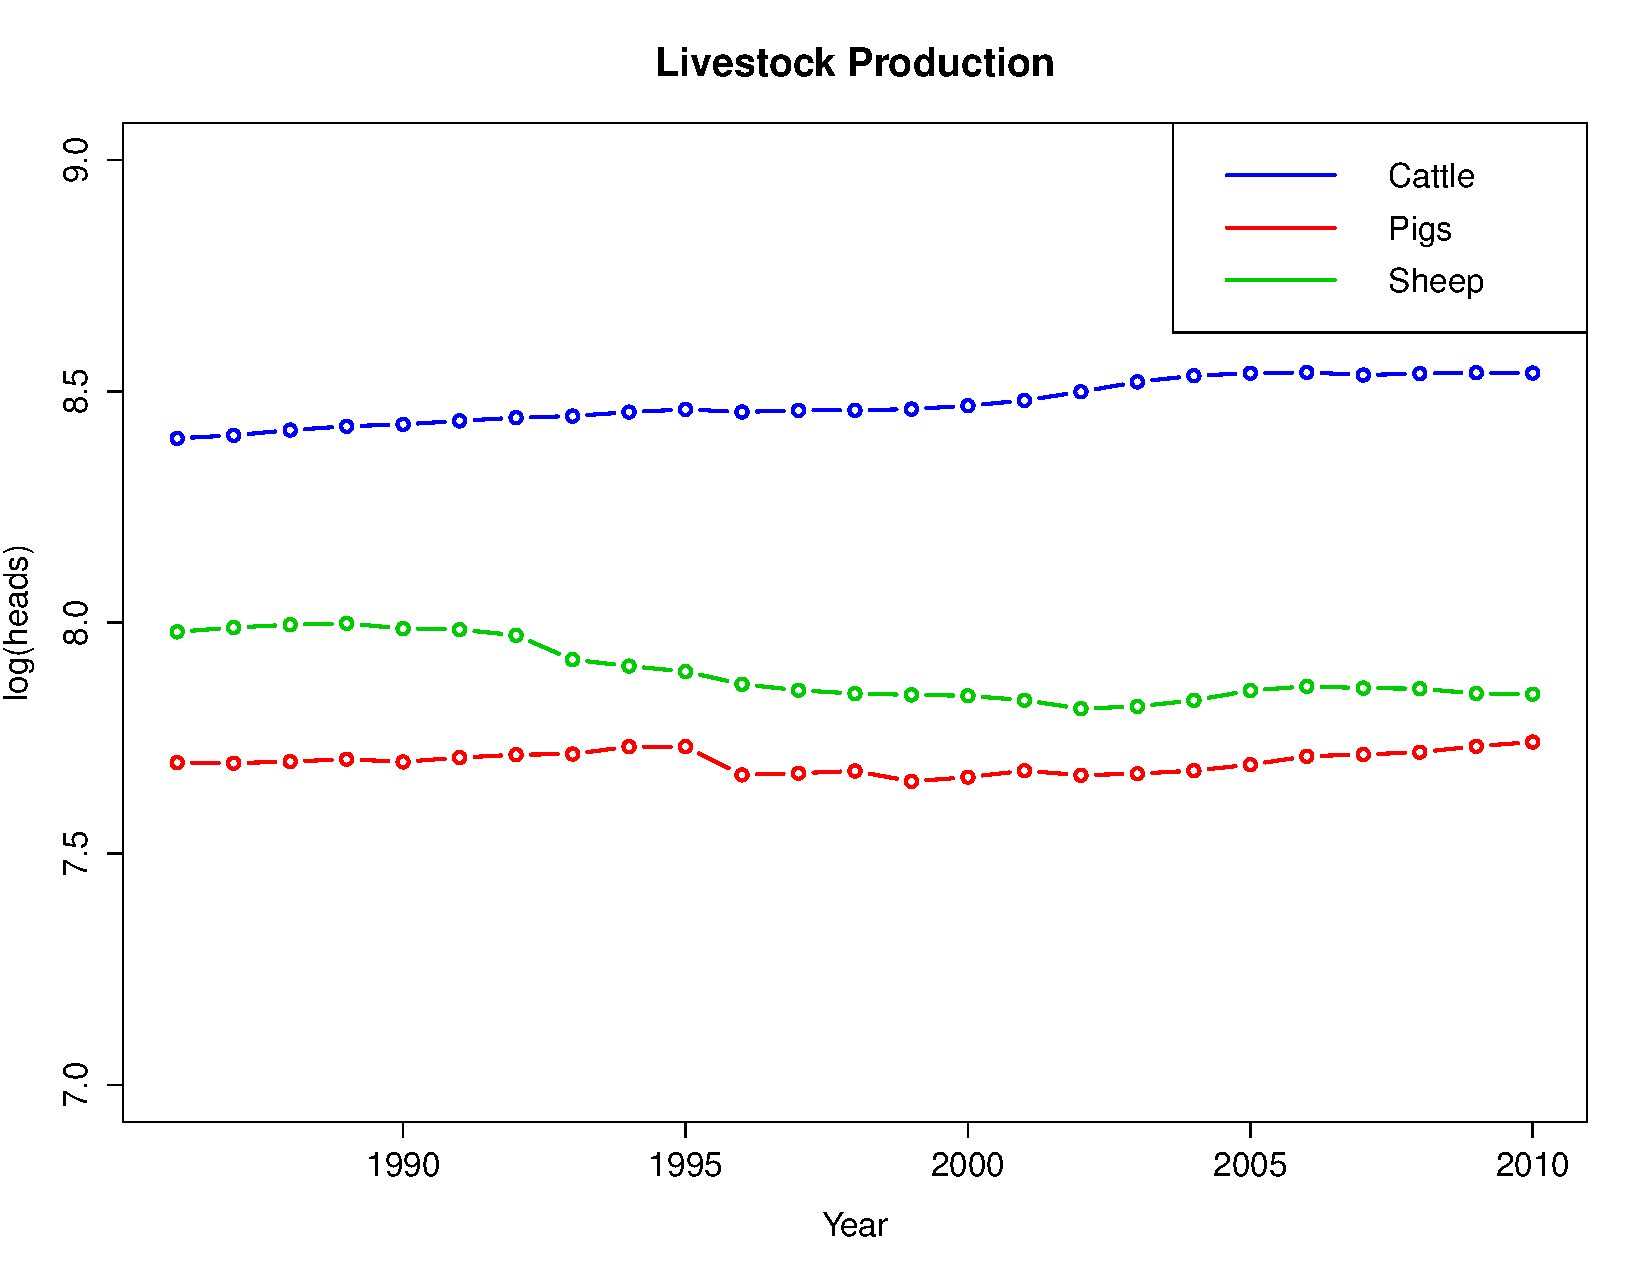
\includegraphics[scale=.250]{FIGURES/production.pdf}}
\end{center}
\caption{}
\label{sfig:trade}
\end{figure}
\end{center}
\newpage
%%%%%%%%%%%%%%%%%%
%%%%%%%%%%%%%%%%%%
\begin{figure}[H]
\begin{center}
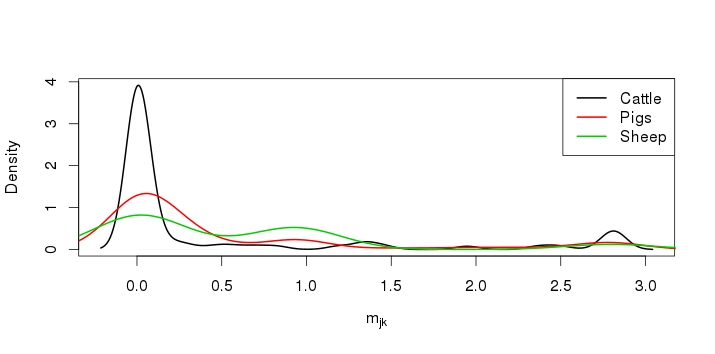
\includegraphics[scale=.5]{FIGURES/trade_info.jpeg}
\end{center}
\caption{}
\label{sfig:tradeinfo}
\end{figure}
\newpage
%%%%%%%%%%%%%%%%%
%%%%%%%%%%%%%%%%%
\begin{figure}[H]
\begin{center}
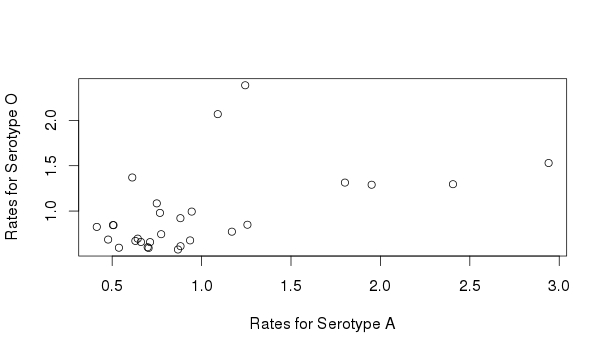
\includegraphics[scale=.5]{FIGURES/A_vs_O_symmetric.jpeg}
\end{center}
\caption{}
\label{sfig:AvsO}
\end{figure}
\newpage
%%%%%%%%%%%%%%%%
%%%%%%%%%%%%%%%%

\begin{figure}[H]
\begin{center}
\subfigure[A]{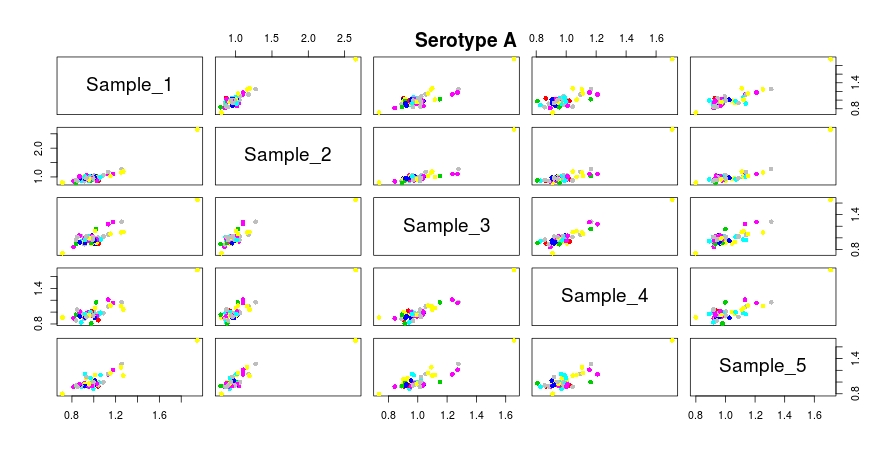
\includegraphics[scale=.250]{FIGURES/rateplot_A.jpeg}}
\subfigure[B]{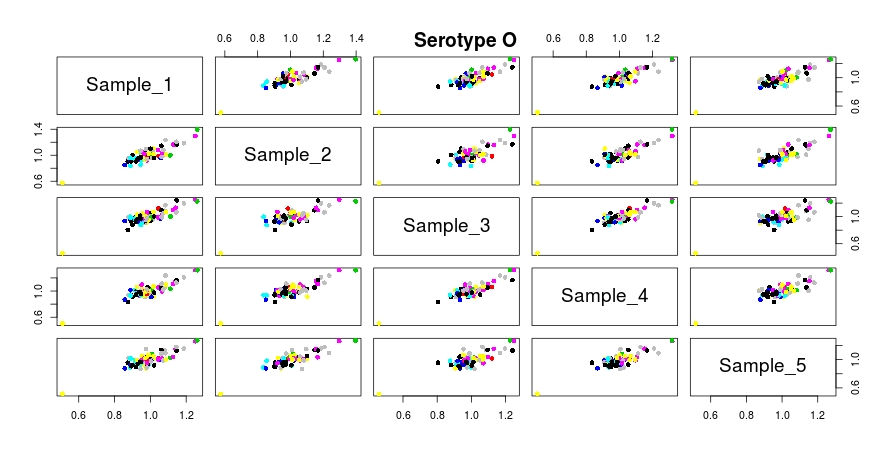
\includegraphics[scale=.250]{FIGURES/rateplot_O.jpeg}}\\
\subfigure[C]{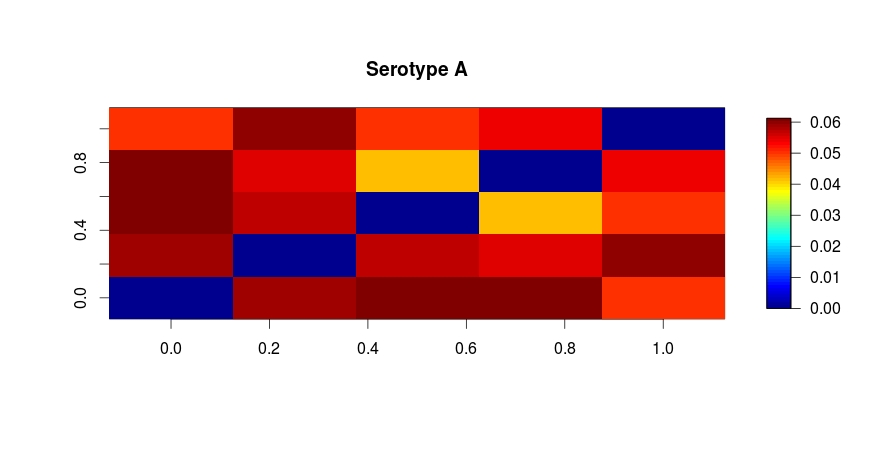
\includegraphics[scale=.250]{FIGURES/normplot_A.jpeg}}
\subfigure[D]{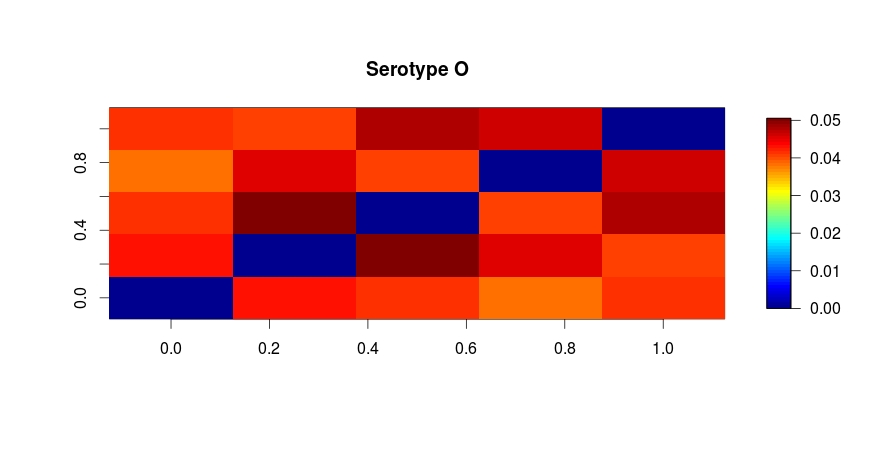
\includegraphics[scale=.250]{FIGURES/normplot_O.jpeg}}%\\
\end{center}
\caption{}
\label{sfig:compz}
\end{figure}
\newpage
%%%%%%%%%%%%%%%%
%%%%%%%%%%%%%%%%
\begin{center}
\begin{figure}[H]
\subfigure[A]{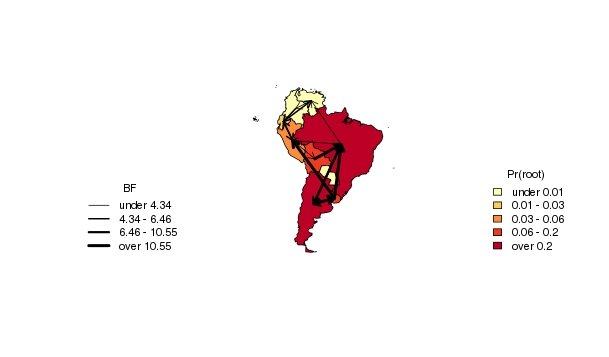
\includegraphics[scale=.350]{FIGURES/A_ss1.jpeg}}
\subfigure[B]{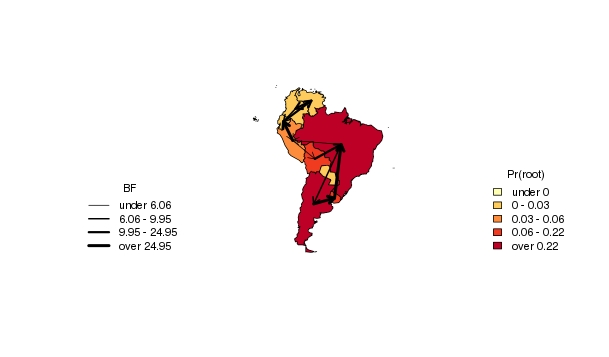
\includegraphics[scale=.350]{FIGURES/A_ss2.jpeg}}\\
\subfigure[C]{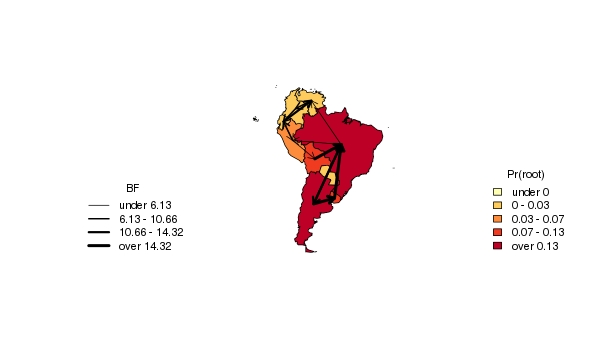
\includegraphics[scale=.350]{FIGURES/A_ss3.jpeg}}
\subfigure[D]{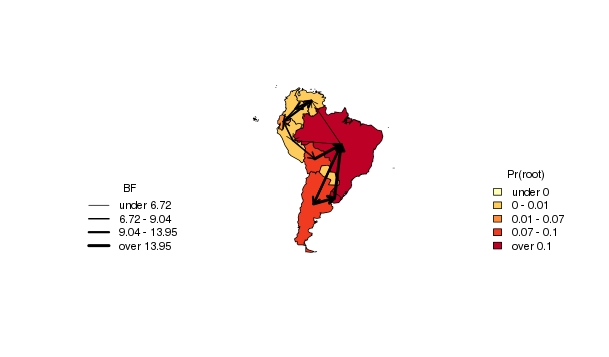
\includegraphics[scale=.350]{FIGURES/A_ss4.jpeg}}\\
\subfigure[E]{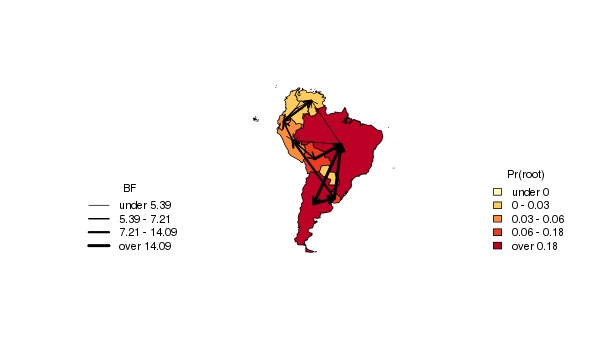
\includegraphics[scale=.350]{FIGURES/A_ss5.jpeg}}
\caption{}
\label{sfig:bssvsA}
\end{figure}
\end{center}
\newpage
%%%%%%%%%%%%%%%
%%%%%%%%%%%%%%%
\begin{figure}[H]
\begin{center}
\subfigure[A]{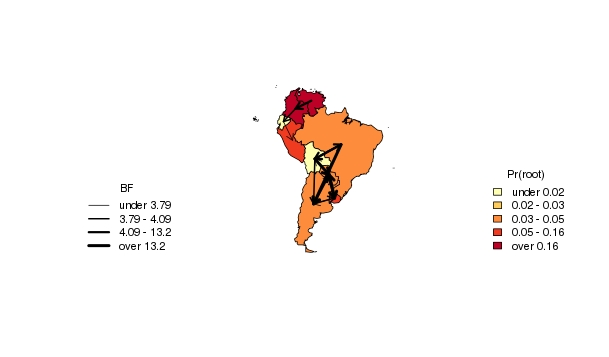
\includegraphics[scale=.250]{FIGURES/O_ss1.jpeg}}
\subfigure[B]{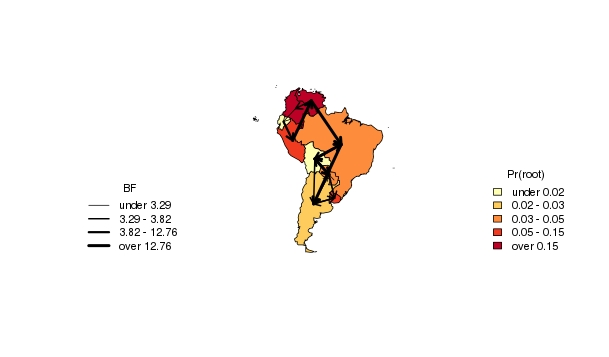
\includegraphics[scale=.250]{FIGURES/O_ss2.jpeg}}\\
\subfigure[C]{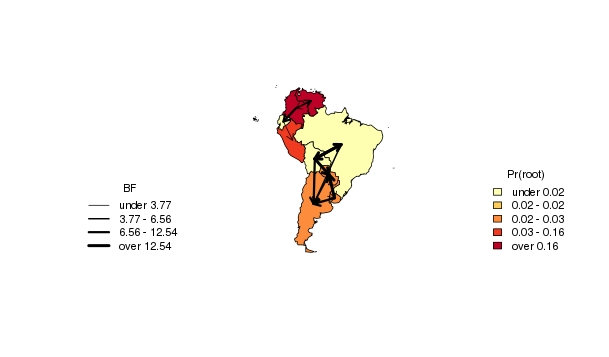
\includegraphics[scale=.250]{FIGURES/O_ss3.jpeg}}
\subfigure[D]{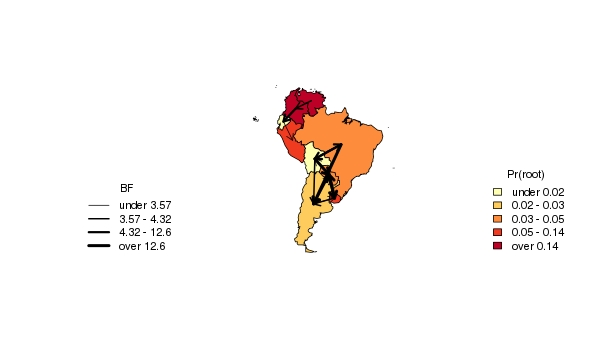
\includegraphics[scale=.250]{FIGURES/O_ss4.jpeg}}\\
\subfigure[E]{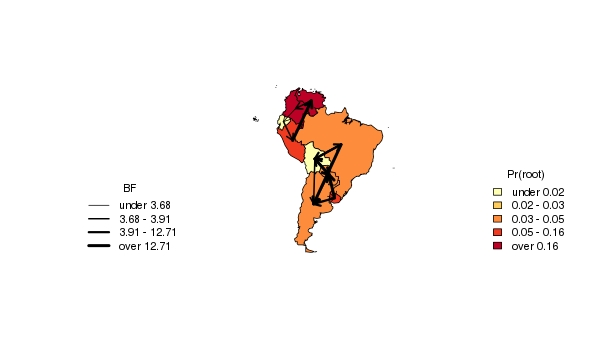
\includegraphics[scale=.250]{FIGURES/O_ss5.jpeg}}
\end{center}
\caption{}
\label{sfig:bssvsO}
\end{figure}
\newpage
%%%%%%%%%%%%%%%%
%%%%%%%%%%%%%%%%
\begin{figure}[H]
\begin{center}
\subfigure[A]{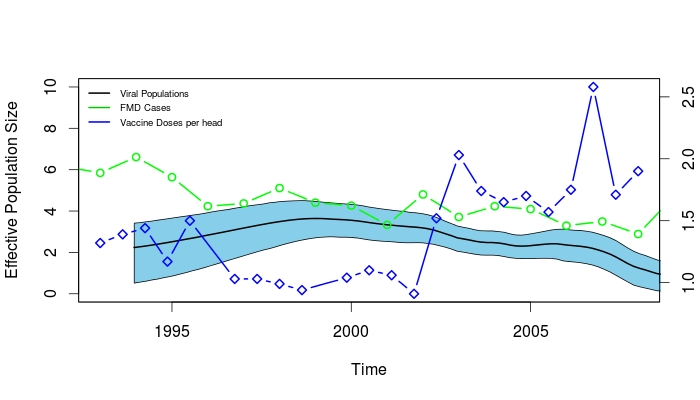
\includegraphics[width=\textwidth]{FIGURES/SFig_A2000sky.jpeg}}
\subfigure[B]{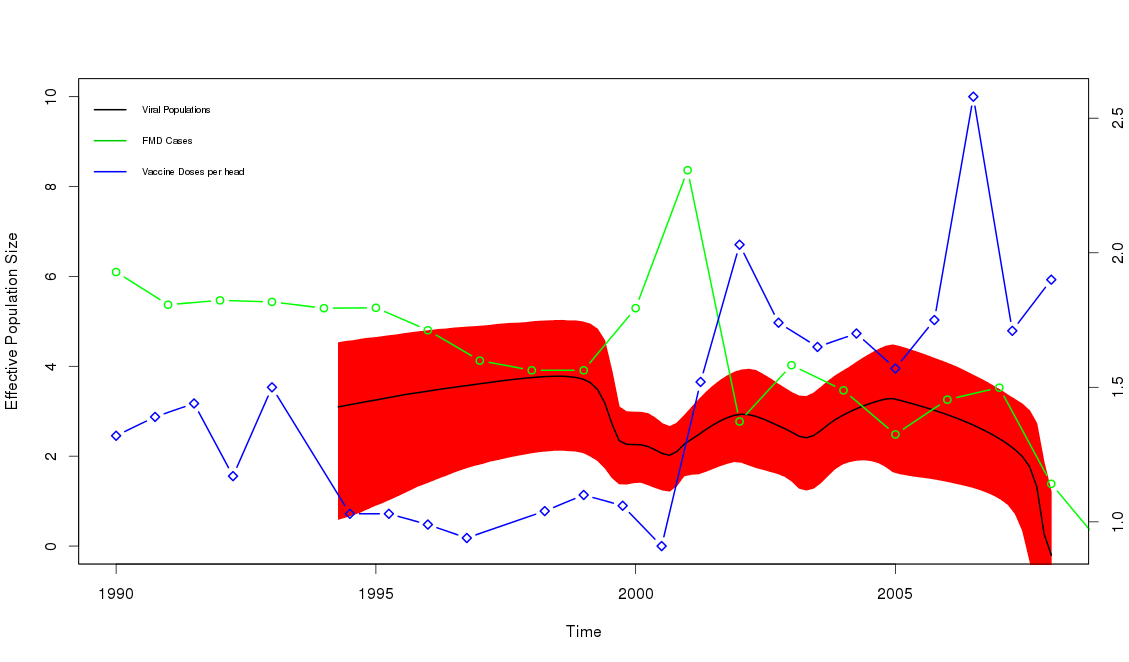
\includegraphics[width=\textwidth]{FIGURES/SFig_O2000sky.jpeg}}\\
\end{center}
\caption{}
\label{sfig:only2000sky}
\end{figure}
\newpage
%%%%%%%%%%%%%%%%
%%%%%%%%%%%%%%%%
\begin{table}[H]
\caption{\textbf{Model selection for tree (coalescent) model and clock for both serotypes.}
ULN= uncorrelated log-normal; UCED = uncorrelated exponential .
Best fitting models (highest log-likelihood) are highlighted in bold.
1- Log-likelihood estimated using Stepping-Stone sampling (SS).}
\begin{center}
\begin{tabular}{cccccc}
\toprule
Serotype	&Coalescent	&Clock	&Log-Likelihood$^{1}$\\
\midrule
A	&Constant	&ULN	&-12285\\
A	&Skyride 	&ULN	&\textbf{-12274}\\
A	&Constant	&UCED	&-12316\\
A	&Skyride 	&UCED	&-12307\\
A       &Skyride       &STRICT &-12308\\
O	&Constant	&ULN	&-8087\\
O	&Skyride 	&ULN	&-8082\\
O	&Constant	&UCED	&-8090\\
O	&Skyride 	&UCED	&\textbf{-8069}\\
O       &Skyride       &STRICT &-8125\\
\bottomrule
\end{tabular}
\end{center}
\begin{flushleft}
\end{flushleft}
\label{stab:treeclockselection}
 \end{table}
 %%%%%%%%%%%%%%%%%%
 %%%%%%%%%%%%%%%%%%
\begin{sidewaystable}[h]
\caption{
\textbf{Spatial signal for FMDV serotypes A and O data sets.} We used Bayesian tip-association significance testing (BaTS) to assess the degree of spatial signal contained in the alignments for both serotypes. 1-Monophyletic clade size}
\begin{tabular}{ccccccc}
\toprule
&\multicolumn{3}{c}{Serotype A} & \multicolumn{3}{c}{Serotype O} \\
MC$^1$ Statistic &Observed mean ( 95\% CI)&Null mean ( 95\% CI)&p-value &Observed mean ( 95\% CI)&Null mean ( 95\% CI)&p-value\\
\midrule
Argentina &12.31 (12.00, 14.00)	&3.45	(2.22, 5.11)	&0.001& 1.00 (1.00, 1.00)&	1.00 (1.00, 1.00)&	1.000\\
Brazil &10.27	(10.00, 11.00)	&2.02 (1.25, 3.00) &0.001& 19.00 (19.00, 19.00)&	2.19 (1.66, 3.03)&	0.001\\
Bolivia &6.00 (6.00, 6.00)	&1.39 (1.00, 2.00)	&0.001&1.00 (1.00, 1.00)&	1.00 (1.00, 1.00)&	1.000\\
Colombia &5.11 (5.00, 6.00)	&1.10  (1.00, 1.99)	&0.001&1.00 (1.00, 1.00)&	1.00 (1.00, 1.00)&	1.000\\
Ecuador &1.00 (1.00, 1.00)	&1.00 (1.00, 1.00)	&1.000&13.00 (13.00, 13.00)&	1.34 (1.00, 2.00)&	0.001\\
Paraguay&-- &-- &--  & 39.40 (31.00, 58.00)& 4.67 (3.43, 6.39)&0.001\\
Peru&1.00 (1.00, 1.00)	&1.02 (1.00, 1.00)&1.000&1.00 (1.00, 1.00)&1.01 (1.00, 1.00)&1.000\\
Uruguay &5.11 (5.00, 7.00)	&1.50	(1.00, 2.03)	&0.001&4.00 (4.00, 4.00)&	1.06 (1.00, 1.32)&	0.001\\
Venezuela&1.82 (1.00, 2.00)	&1.02 (1.00, 1.08)	&0.010&6.00 (6.00, 6.00)&	1.28 (1.00, 2.00)&	0.001\\
\bottomrule
\end{tabular}
\begin{flushleft}
\end{flushleft}
\label{stab:BaTS}
\end{sidewaystable}
%%%%%%%%%%%%%
%%%%%%%%%%%%%
\begin{table}[h]
\caption{ {{\bf Parameter estimation using the complete and without Argentina data sets for serotype A.}} To assess the impact of the overrepresentation of Argentina in our sample we removed all sequence from this location and reestimated parameters.
1- All 131 sequences were used. 2- Time to most recent common ancestor. 3- Codon positions $1$, $2$ and $3$. }
\begin{center}
\begin{tabular}{ccc}
\toprule
Parameter	&Complete$^{1}$	&Without Argentina\\
\midrule
TMRCA$^{2}$	&76.40 (69.48-83.65)	&82.31 (72.40-92.81)\\
CP1$	^{3}$	&0.65 (0.54-0.76)	&0.62 (0.51-0.75)\\
CP2	&0.46 (0.37-0.58)	&0.41 (0.31-0.53)\\
CP3	&1.87 (1.74-2.00)	& 1.95 (1.81 -2.09)\\
Rate ($\times 10^{-3}$)	&4.14 (3.39-4.98)	&3.46 (2.82-4.11)\\
\bottomrule
\end{tabular}
\end{center}
\label{stab:SB_A}
 \end{table}
%%%%%%%%%
%%%%%%%%%
\begin{table}[h]
\caption{ {{\bf Parameter estimation using the complete and without Ecuador data sets for serotype O.}} To assess the impact of the overrepresentation of Ecuador (90 sequences) our sample we removed all sequence from this location and reestimated parameters.
1- All 167 sequences were used. 2- Time to most recent common ancestor. 3- Codon positions $1$, $2$ and $3$.
}
\begin{center}
\begin{tabular}{ccc}
\toprule
Parameter	&Complete$^{1}$	&Without Ecuador\\
\midrule
TMRCA$^{2}$	&21.25 (19.20-23.60)	&22.65 (17.6-29.5)\\
CP1$^{3}$	&0.51 (0.39-0.63)	&0.51 (0.39-0.64)\\
CP2	&0.53 (0.39-0.69)	&0.42 (0.29-0.59)\\
CP3	&1.94 (1.78-2.10)	& 2.05 (1.87 -2.21)\\
Rate ($\times 10^{-2}$)	&1.11 (0.91-1.32)	&0.91 (0.63-1.21)\\
\bottomrule
\end{tabular}
\end{center}
\label{stab:SB_O}
 \end{table}

%%%%%%%%
%%%%%%%%
\newpage
\begin{sidewaystable}
\medskip
\begin{minipage}{\textwidth} 
\begin{center}
\caption{ {{\bf 'Equal down-sampling' experiment for serotype A.}} 
Five random down-sampled subsamples were obtained and used for parameter inference.
1-- $\times 10^{-3}$; 2 -- $\times 10^{-2}$; 3-- Probability distribution at root node; 4-- Kullback-Leibler Divergence (see Text) }
\begin{tabular}{cccccc}
\toprule
Subsample	&mean subs. rate$^{1}$ (95 \% BCI)	&TMRCA (95 \% BCI)	&mean migration rate$^{2}$  (95 \% BCI)	&Root (Pr$^{3}$)& KL$^4$\\
\midrule
1	&4.21 (3.43-5.05)	&78.97 (71.21-86.82)	&2.63 (1.34-4.08)	&Argentina (0.41)& 1.76\\
2	&4.25 (3.44-5.07)	&79.64 (71.49-88.04)	&2.54 (1.28-3.98)	&Brazil (0.40)& 1.41\\
3	&4.12 (3.38-4.94)	&77.74 (70.26-85-86)	&2.49 (1.27-3.88)	&Brazil (0.57)&1.47\\
4	&4.12 (3.41-4.82)	&77.60 (69.41-85.88)	&2.44 (1.21-3.85)	&Brazil (0.61)&0.98\\
5	&4.19 (3.49-4.93)	&78.28 (70.23-86.96)	&2.66 (1.31-4.11)	&Brazil (0.45)& 1.00\\
\bottomrule
\end{tabular}
\label{stab:ED_A}
\end{center}
\end{minipage}
\end{sidewaystable}

%%%%
%%%%
\newpage
\begin{sidewaystable}
\medskip
\begin{minipage}{\textwidth}
\begin{center}
 \caption{ {{\bf 'Equal down-sampling' experiment for serotype O.}} Five random down-sampled subsamples were obtained and used for parameter inference.
1-- $\times 10^{-3}$; 2--  Probability at root node; 3-- Kullback-Leibler Divergence (see Text).}
\begin{tabular}{cccccc}
\toprule
Subsample	&mean subs. rate$^{1}$ (95 \% BCI)	&TMRCA (95 \% BCI)	&mean migration rate$^{1}$ (95 \% BCI)	&Root (Pr$^{2}$) & KL$^3$\\
\midrule
1	&1.11 (0.86-1.37)	&20.27 (18.45-21.95)	&8.48 (3.91-13.59)	&Venezuela (0.45)& 1.24\\
2	&0.865 (0.62-1.11)	&22.40 (19.78-25.31)	&8.74 (3.84-14.28)	&Venezuela (0.46)&1.04\\
3	&0.94 (0.68-1.21)	&21.91 (19.46-24.56)	&8.72 (4.03-14.17)	&Venezuela (0.51)&1.52\\
4	&0.84 (0.62-1.18)	&22.54 (19.80-25.45)	&8.43 (3.77-13.67)	&Venezuela (0.49)&1.00\\
5	&0.88 (0.63-1.13)	&22.33 (19.55-25.26)	&8.58 (3.89-13.18)	&Venezuela (0.44)&1.23\\

\bottomrule
\end{tabular}
\label{stab:ED_O}
\end{center}
\end{minipage}
\end{sidewaystable}
%%%%
%%%%
\end{document}
